\chapterimage{chap39.jpg}
\chapter{Summary}

\section{柯西收敛准则}

\begin{theorem}[柯西收敛准则]\label{the: 柯西收敛准则}
	柯西极限存在准则, 又称柯西收敛准则, 给出某个式子(数列、数项级数、函数等)收敛的一个充分必要条件, 主要应用在数列、数项级数、函数、反常积分、函数列和函数项级数等的收敛性判断中
\end{theorem}

\begin{proposition}[柯西收敛准则:数列]
	数列 $\{a_{n}\}$ 收敛的充分必要条件
	$$\forall \varepsilon > 0, \exists N \in \mathbb{N}^{+},\ s.t.\ n,m > N, |a_{n} - a_{m}| < \varepsilon$$
	满足条件的 $\{a_{n}\}$ 称为柯西序列, 上述定理也可表述为: 数列 $\{a_{n}\}$ 收敛当且仅当 $\{a_{n}\}$ 是柯西序列
\end{proposition}

\begin{anymark}[证明]
	(1). 必要性:

	不妨设 $\lim\limits_{n\to \infty} a_{n} =\eta$, 对于任意 $\varepsilon > 0$, 存在 $N_{0}\in\mathbb{N}$, 当 $n>N_{0}$ 时, $|a_{n}-\eta|<\dfrac{\varepsilon}{2}$, 我们有:
	$$\begin{cases} 
		\forall n > N_{0}, s.t.\ |a_{n} - \eta| < \dfrac{\varepsilon}{2}\\ 
		\forall m > N_{0}, s.t.\ |a_{m} - \eta| < \dfrac{\varepsilon}{2}
	\end{cases}
	\Rightarrow 
	|x_{n}-x_{m}| = |(x_{n} - \eta) - (x_{m} - \eta)| \leq |x_{n} - \eta| + |x_{m}-\eta| \leq \varepsilon$$

	(2). 充分性:


\end{anymark}

\begin{proposition}[柯西收敛准则:数项级数]
	数项级数收敛的充要条件:
	$$\forall \varepsilon > 0, \exists N \in \mathbb{N}^{+},\ s.t.\ m > n > N, |u_{n+1} + u_{n+2} + \cdots + u_{m}| < \varepsilon$$
\end{proposition}

\begin{anymark}[证明]
	不妨设数项级数 $\sum\limits_{n = 1}^{+\infty}u_{n}$ 的部分和为 $S_{n}$, 
	$\sum\limits_{n = 1}^{+\infty}u_{n}$ 收敛当且仅当 $\lim\limits_{n \to +\infty}S_{n}$ 存在

	数列的柯西收敛准则:

	$$\forall \varepsilon > 0, \exists N \in \mathbb{N}^{+},\ s.t.\ n,m > N, |S_{n} - S_{m}| = |u_{n+1} + u_{n+2} + \cdots + u_{m}| < \varepsilon$$
\end{anymark}

\begin{proposition}[柯西收敛准则:函数]
	(1). $\lim\limits_{x \to x_{0}}f(x)$ 收敛的充要条件:

	$$\forall \varepsilon > 0, \exists \delta > 0,\ s.t.\ x_{1},x_{2}\in \mathring{U}(x_{0},\delta), |f(x_{1})-f(x_{2})| < \varepsilon$$

	(2). $\lim\limits_{x \to \infty}f(x)$ 收敛的充要条件:

	$$\forall \varepsilon > 0, \exists X > 0,\ s.t.\ |x_{1}|,|x_{2}| > |X|, |f(x_{1})-f(x_{2})| < \varepsilon$$
\end{proposition}
\begin{proposition}[柯西收敛准则:反常积分]
	1. 无穷积分

	(1). $\int_{a}^{+\infty}f(x)dx$ 收敛的充要条件:

	$$\forall \varepsilon > 0, \exists X > 0,\ s.t.\ q > p > X([p,q]\subset [a,+\infty)), |\int_{p}^{q}f(x)dx| < \varepsilon$$

	(2). $\int_{-\infty}^{a}f(x)dx$ 收敛的充要条件:

	$$\forall \varepsilon > 0, \exists X > 0,\ s.t.\ p < q < -X([p,q]\subset (-\infty,a]), |\int_{p}^{q}f(x)dx| < \varepsilon$$


	2. 暇积分

	(1). $\int_{a}^{b}f(x)dx$ 收敛的充要条件:($x = a$ 是瑕点)

	$$\forall \varepsilon > 0, \exists \delta > 0,\ s.t.\ a < p < q < a + \delta ([p,q]\subset [a,b]), |\int_{p}^{q}f(x)dx| < \varepsilon$$

	(2). $\int_{a}^{b}f(x)dx$ 收敛的充要条件:($x = b$ 是瑕点)

	$$\forall \varepsilon > 0, \exists \delta > 0,\ s.t.\ b - \delta < p < q < b ([p,q]\subset [a,b]), |\int_{p}^{q}f(x)dx| < \varepsilon$$
\end{proposition}

\begin{proposition}[柯西收敛准则:函数列和函数项级数]
	
\end{proposition}

\section{双曲函数}

\begin{figure}[htbp]
	\centering
	\includegraphics[width=9.5cm,height=8cm]{"figure/Summary/双曲函数.png"}
	\caption{双曲函数示意图}
	\label{Figure: 双曲函数示意图}
\end{figure} 
\begin{definition}[双曲函数]\label{def: 双曲函数}
	双曲函数是一种类似于三角函数的一类函数, 基本的函数有双曲正弦函数和双曲余弦函数, 借由指数函数定义
	
	1. 双曲正弦函数 
	$$\sinh x=\frac{e^{x}-e^{-x}}{2},x\in \mathbb{R}\quad \mathbb{R}\rightarrow \mathbb{R}$$
	
	2. 双曲余弦函数
	$$\cosh x=\frac{e^{x}+e^{-x}}{2},x\in \mathbb{R}\quad \mathbb{R}\rightarrow [1,+\infty]$$
	
	3. 双曲正切函数
	$$\tanh x=\frac{e^{x}-e^{-x}}{e^{x}+e^{-x}},x\in \mathbb{R}\quad \mathbb{R}\rightarrow (-1,1)$$
	
	恒等式:  
	$$\cosh^2 x-\sinh^2=1$$
	$$\sinh x=-i\sin ix,\quad \cosh x=\cos ix$$
	$$\sinh x=\sum\limits_{n=0}^{+\infty}\frac{x^{2n+1}}{(2n+1)!}=x+\frac{x^3}{3!}+\frac{x^5}{5!}+\dots$$
	$$\cosh x=\sum\limits_{n=0}^{+\infty}\frac{x^{2n}}{2n!}=1+\frac{x^2}{2!}+\frac{x^4}{4!}+\dots$$
\end{definition}
\begin{definition}[反双曲函数]
	1. 反双曲正弦函数
	$$\arsinh x=ln(x+\sqrt{x^2+1}),\quad (arsinh x)'=\frac{1}{\sqrt{x^2+1}}$$
	
	2. 反双曲余弦函数
	$$\arcosh x=ln(x+\sqrt{x^2-1}),\quad (arcosh x)'=\frac{1}{\sqrt{x^2-1}}$$
	
	3. 反双曲正切函数
	$$\artanh x=\frac{1}{2}ln(\frac{1+x}{1-x}),\quad (artanh x)'=\frac{1}{1-x^2}$$
\end{definition}

\section{两类欧拉积分}

\begin{definition}[$Gamma$ 函数和 $Beta$函数]	
	1. $Gamma$ 函数(欧拉第一类积分)

	$$B(p,q) = \int_{0}^{1}x^{p-1}(1-x)^{q-1}dx=B(q,p)$$
	
	$$B(a,b) = (\dfrac{x^a(1-x)^b}{a})\big|_{0}^{1} + \dfrac{b-1}{a}\int_{0}^{1}x^{a}(1-x)^{b-2}dx$$
	$$B(a,b) = \dfrac{b-1}{a}\int_{0}^{1}(x-1+1)x^{a-1}(1-x)^{b-2}$$
	$$\mathcolorbox{yellow}{B(a,b) = \dfrac{b-1}{a}[B(a,b-1)-B(a,b)]}$$ 
	
	$$\mathcolorbox{yellow}{B(a,b) = \dfrac{b-1}{a+b-1}B(a,b-1)}$$
	
	特别的:  $$\mathcolorbox{yellow}{B(m,n) = \dfrac{(n-1)!(m-1)!}{(m+n-1)!}}$$
	
	2.$Beta$函数(第二类欧拉积分)

	$$\Gamma(\alpha) = 
	\begin{cases} 
		\int_{0}^{+\infty}x^{\alpha-1}e^{-x}dx\\ 
		2\int_{0}^{+\infty}x^{2\alpha-1}e^{-x^{2}}dx
	\end{cases}$$
	
	$$\Gamma(\alpha) = (-x^{\alpha-1}e^{-x})\big|_{0}^{+\infty}+(\alpha-1)\int_{0}^{+\infty}x^{\alpha-2}e^{-x}dx$$
	
	$$\mathcolorbox{red}{\Gamma(\alpha) = (\alpha-1)\Gamma(\alpha-1)} (\alpha>1)$$

	有两个特别的 $\alpha$, 分别是 $\alpha = \dfrac{1}{2}$ 和 $\alpha = 1$:

	$$\begin{cases} 
		\int_{0}^{+\infty}e^{-x}dx = 1 & \alpha =1 \\ 
		\int_{0}^{+\infty}x^{-\frac{1}{2}}e^{-x}dx = 2\int_{0}^{+\infty}e^{-x^{2}}dx = \sqrt{\pi} & \alpha =\dfrac{1}{2}
	\end{cases}$$
	
	特别的  $$\mathcolorbox{red}{\Gamma(n+1)=n!}$$
	
	3. 两类积分之间的关系
	
	转换公式:  
	$$B(a,b)=\frac{\Gamma(a)\Gamma(b)}{\Gamma(a+b)}$$
	
\end{definition}

\section{多项式函数极值点和拐点}


\begin{theorem}[代数基本定理]\label{the: 代数基本定理}
	任何一个一元 $n$ 次复系数多项式, 都恰好有 $n$ 个复根, 且可以表示为 $n$ 个一次因式的乘积
\end{theorem}

\begin{corollary}[曲线的极值点和拐点]
	曲线上的可导点不可能同时是极值点和拐点, 不可导点可能同时是极值点和拐点
\end{corollary}

\begin{proposition}[多项式函数极值点和拐点个数:命题一]\label{pro: 命题一}
	多项式函数 $f(x) = (x-a)^{n}(n>1)$, 当 $n$ 为奇数时, $(a,0)$ 是 $f(x)$ 的拐点, 当 $n$ 为偶数时, $x=a$ 是 $f(x)$ 的极值点
\end{proposition}
\begin{anymark}[证明]

	$$\begin{cases}
		f'(x) = n(x-a)^{n-1}\\
		f''(x) = n(n-1)(x-a)^{n-2}
	\end{cases}$$

	当 $n$ 为偶数时, $f'(a) = 0$ 且 

	$$\exists \delta > 0, x\in (a-\delta,a),f'(x)<0; x\in (a,a+\delta),f'(x)>0$$
	
	当 $n$ 为偶数时, $x=a$ 是 $f(x)$ 的极值点
	
	当 $n$ 为奇数时, $f''(a) = 0$ 且
	
	$$\exists \delta > 0, x\in (a-\delta,a),f''(x)<0; x\in (a,a+\delta),f''(x)>0$$

	当 $n$ 为奇数时, $(a,0)$ 是 $f(x)$ 的拐点
	

\end{anymark}


\begin{proposition}[多项式函数极值点和拐点个数:命题二]\label{pro: 命题二}
	多项式函数 $f(x) = (x-a)^{n}g(x)(n>1), g(a)\neq 0$, 当 $n$ 为奇数时, $(a,0)$ 是 $f(x)$ 的拐点, 当 $n$ 为偶数时, $x=a$ 是 $f(x)$ 的极值点
\end{proposition}
\begin{anymark}[证明]

	$$\begin{cases}
		f'(x) = (x-a)^{n-1} \left[ ng(x) + (x-a)g'(x) \right]\\
		f''(x) = (x-a)^{n-2} \left[ n(n-1)g(x) + 2n(x-a)g'(x) + (x-a)^{2}g''(x) \right]
	\end{cases}$$

	当 $n$ 为偶数时, 不妨假设 $g(a) > 0$, 极限的保号性:
	
	$$\exists \delta_{1} > 0, s.t.\ x\in U(a,\delta_{1}), g(a) > 0$$
	
	当 $x\in U(a,\delta_{1}), f(x) = (x-a)^{n}g(x) \geq f(a) = 0$, $x=a$ 是 $f(x)$ 的一个极值点


	当 $n$ 为奇数时, $x\to a,(x-a),(x-a)^{2}$ 是无穷小量, $g'(a),g''(a)$ 都是定值

	$$\exists \delta_{2} > 0, s.t.\ x\in U(a,\delta_{2}), 2n(x-a)g'(x)+(x-a)^{2}g''(x)\leq |n(n-1)g(x)| $$

	$x\in U(a,\delta_{2}), \left[ n(n-1)g(x) + 2n(x-a)g'(x) + (x-a)^{2}g''(x) \right] > 0$, $f''(x)$ 与 $(x-a)^{n-2}$ 符号相同

	当 $x\in (a-\delta_{2},a), f''(x) < 0; x\in (a,a+\delta_{2}), f''(x) > 0$, $(a,0)$ 是 $f(x)$ 的一个拐点
\end{anymark}

\begin{proposition}[多项式函数极值点和拐点个数:命题三]\label{pro: 命题三}
	讨论多项式函数 $P_{n}(x) = \prod\limits_{i = 1}^{k}(x-a_{i})^{p_{i}}$ 极值点和拐点个数,其中满足:
	$$p_{i}\in\mathbb{Z}^{+}, p_{1} < p_{2} < \cdots < p_{k}, a_{i}\in \mathbb{R}$$
\end{proposition}
\begin{corollary}[极值点和拐点个数]
	假设 $P_{n}(x) = \prod\limits_{i = 1}^{k}(x-a_{i})^{p_{i}}$, 其中 $k_{1}$ 个 $p_{i}$ 为奇数(大于 $1$), $k_{2}$ 个 $p_{i}$ 为偶数, $k_{0}$ 个 $p_{i}=1$, 满足 $k_{0}+k_{1}+k_{2} = k$
	\begin{itemize}
		\item $P_{n}(x)$ 的极值点个数 $k-1+k_{2} = k_{0}+k_{1}+2k_{2}-1$
		\item $P_{n}(x)$ 的拐点个数 $k+2k_{1}+k_{2}-2 = k_{0}+3k_{1}+2k_{2}-2$
	\end{itemize}
\end{corollary}
\begin{anymark}[证明]

	(1). 极值点个数

	$P_{n}(x)$ 是多项式函数, 在 $\mathbb{R}$ 上 $n$ 阶可导
	
	$$\begin{cases}
	  P_{n}(x) \text{极值点满足: } P_{n}'(x) = 0\\
	  P_{n}(x) \text{拐点满足: } P_{n}''(x) = 0
	\end{cases}$$

	$P(x)$ 有 $k$ 个实数根, $k$ 个实数根的重数分别为 $p_{1},p_{2},\cdots,p_{k}$, 且 $\sum\limits_{i = 1}^{k}p_{i}= n$

	不妨设 $\begin{cases}
		k_{0} = N(p_{i} = 1)\\
		k_{1} = N(p_{i} \in \{2k + 1, k \in \mathbb{Z}^{+}\})\\
		k_{2} = N(p_{i} \in \{2k, k \in \mathbb{Z}^{+}\})
	\end{cases}$

	$$P_{n}'(x) =  \prod\limits_{i = 1}^{k}(x-a_{i})^{p_{i}-1} \left[\sum\limits_{i = 1}^{k}p_{i} \left(\prod\limits_{\substack{j = 1 \\ j\neq i}}^{k}(x - a_{j})\right)\right]$$

	当 $p_{i} \geq 2(i = k_{0} + 1, k_{0} + 2,\cdots,k)$ 时, $x = a_{i}$ 是 $P_{n}'(x)$ 的一个零点,
	此类零点一共有 $k - k_{0}$ 个, $P_{n}'(x)$ 有 $p_{i}-1$ 重根 $a_{i}$

	$P_{n}'(x)$ 此类的零点个数为 $n_{1} = \sum\limits_{i = k_{0} + 1}^{k}(p_{i}-1) = n-k$
	
	将 $P(x)$ 的 $k$ 个零点按照从小到大排列: $a_{1}, a_{2},\cdots,a_{k}$

	罗尔定理:
	
	$$\exists \xi_{i} \in (a_{i},a_{i+1})(i = 1, 2, \cdots, k-1),\ s.t.\ P'(\xi_{i}) = 0$$
	
	$P_{n}'(x)$ 此类的零点个数为 $n_{1} = k - 1$ 个; $P'_{n}(x)$ 是 $n-1$ 次多项式函数, 至多有 $n-1$ 个复根, 
	$P'_{n}(x)$ 有 $n-k+k-1 = n-1$ 个实数根, 其中前面 $n-k$ 个根中存在重根情况

	\begin{corollary}[多项式函数零点]
		$P_{n}(x)$ 有 $n$ 个实数根(含重根), 那么 $P_{n}'(x),P_{n}''(x),\cdots,P_{n}^{(n-1)}(x)$ 的根全部是实数
	\end{corollary}

	$P_{n}'(x)$ 的两类零点
	
	$$P'_{n}(x) = \prod\limits_{i = 1}^{k}(x - a_{i})^{p_{i} - 1}f(x)$$
	
	第一类零点:
	
	$\mathbf{pro}$ \ref{pro: 命题二}: 当 $p_{i}$ 为偶数, $a_{i}$ 是 $P_{n}(x)$ 的极值点, 共有 $k_{2}$ 个极值点
	
	第二类零点: 
	
	$f(\xi_{i}) = 0 (\xi_{i}\in (a_{i},a_{i+1}))$, 当 $x\in U(\xi_{i},\delta)$ 时, 只有 $(x-\xi_{i})$ 这一项符号改变, 
	因此 $x=\xi_{i}$ 是 $P_{n}(x)$ 极值点, 共有 $k - 1$ 个极值点
	
	综上, $P_{n}(x)$ 的极值点个数为 $k - 1 + k_{2} = k_{0} + k_{1} + 2k_{2} - 1$


	(2). 拐点个数
	
	类比极值点个数的方法, 求 $P'_{n}(x)$ 极值点个数
	
	$$P_{n}'(x) = \sum\limits_{i=1}^{k}p_{i}\left[(x-a_{1})^{p_{1}-1}(x-\xi_{1})(x-a_{2})^{p_{2}-1}\cdots(x-\xi_{k-1})(x-a_{k})^{p_{k}-1}\right]$$

	$P'_{n}(x)$ 的极值点有两类:
	
	i. 第一类是 $P'_{n}(x)$ 相邻两个零点之间的点, 也是 $P_{n}''(x)$ 的极值点, 共有 $k_{1} + k_{2} + k - 2$ 个
	
	ii. 第二类是 $P'_{n}(x)$ 的部分零点, 也是 $P_{n}''(x)$ 的极值点, 当 $p_{i} - 1$ 为偶数, $x = a_{i}$ 是 $P_{n}''(x)$ 的极值点, 共有 $k_{1}$ 个
	
	综上, $P_{n}(x)$ 的拐点个数为 $k + 2k_{1} + k_{2} - 2$
\end{anymark}

\section{阿达玛不等式}

\begin{figure}[H]
	\centering
	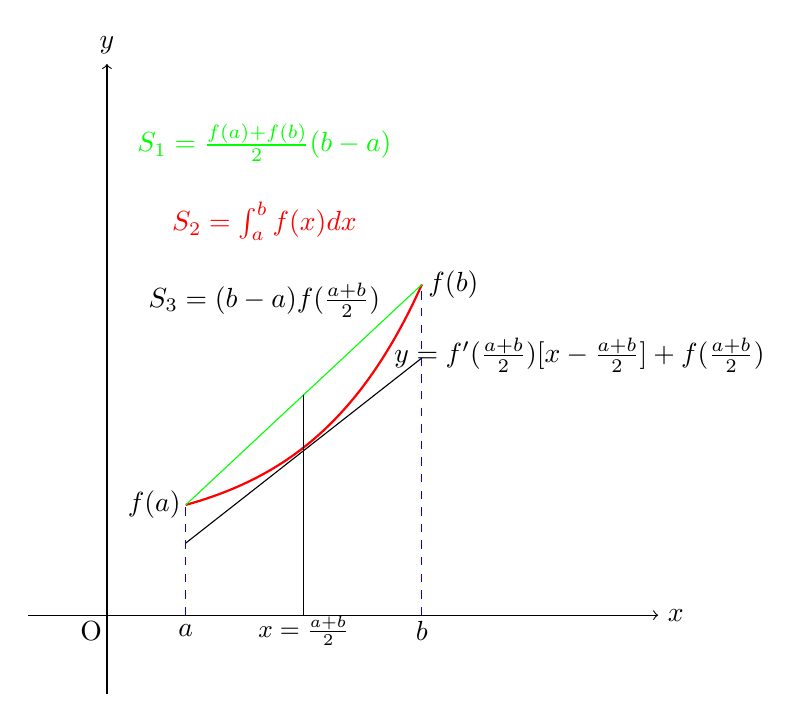
\begin{tikzpicture}
		\draw[->] (-1,0) -- (7,0) node[right] {$x$};
		\draw[->] (0,-1) -- (0,7) node[above] {$y$};
		\draw[red,thick, domain=1:4, smooth, variable=\x] plot ({\x},{0.2*2^(\x)+1});
		\draw[green] (1,1.4) -- (4,4.2);
		\draw (2.5,0) -- (2.5,2.8);
		\draw[dashed,blue] (1,0) -- (1,1.4);
		\draw[dashed,blue] (4,0) -- (4,4.2);
		\draw (1,0.9148) -- (4,3.2668);
		\node at (6,3.3) {$y = f'(\frac{a+b}{2})[x-\frac{a+b}{2}]+f(\frac{a+b}{2})$};
		\node at (1,-0.2) {$a$};
		\node at (4,-0.2) {$b$};
		\node at (2.5,-0.2) {\small{$x=\frac{a+b}{2}$}};
		\node at (0.6,1.4) {$f(a)$};
		\node at (4.4,4.2) {$f(b)$};
		\node at (-0.2,-0.2) {O};
		\node[green] at (2,6) {$S_{1} = \frac{f(a)+f(b)}{2}(b-a)$};
		\node[red] at (2,5) {$S_{2} = \int_{a}^{b}f(x)dx$};
		\node at (2,4) {$S_{3} = (b-a)f(\frac{a+b}{2})$};
	\end{tikzpicture}
	\caption{$Hadamard$不等式}
	\label{Figure: 阿达玛不等式}
\end{figure}

\begin{theorem}[$\mathbf{Hadamard}$不等式]\label{thm: 阿达玛不等式}

	$f(x)$在$[a,b]$上具有二阶导数,且$f''(x)\geq 0$,下面不等式成立:  
	$$f(\dfrac{a+b}{2})\leq \dfrac{1}{b-a}\int_{a}^{b}f(t)dt\leq \dfrac{1}{2}[f(a)+f(b)]$$
	\begin{proof}
		
		原不等式可以化为:  
		$$(b-a)f(\dfrac{a+b}{2})\leq\int_{a}^{b}f(t)dt\leq\dfrac{b-a}{2}[f(a)+f(b)]$$
		
		我们由图\ref{Figure: 阿达玛不等式}可以发现:  
		
		不等式左边表示的过$(\dfrac{a+b}{2},f(\dfrac{a+b}{2}))$的切线与$x=a,x=b,y=0$围成的图形的面积$S_{3}$;
		
		不等式中间表示的是$f(x)$与$x=a,x=b,y=0$围成的曲边梯形的面积$S_{2}$;
		
		不等式右边表示的是直线$x=a,x=b,y=0$与直线$y=\dfrac{f(b)-f(a)}{b-a}(x-a)+f(a)$围成的梯形的面积$S_{1}$.
		
		我们可以由图形上直观的看出三个面积的大小关系:  $S_{3}\leq S_{2}\leq S_{1}$
		
		对于左边的不等式,我们将$f(x)$在$x=\dfrac{a+b}{2}$处展开得到:  
		$$f(x)=f(\dfrac{a+b}{2})+f'(\dfrac{a+b}{2})(x-\dfrac{a+b}{2})+f''(\xi)(x-\dfrac{a+b}{2})^2$$
		
		我们由$f''(x)>0$,我们可以得到:  
		$$f(x)>f(\dfrac{a+b}{2})+f'(\dfrac{a+b}{2})(x-\dfrac{a+b}{2})$$
		
		两边同时在$[a,b]$内取定积分得到:  
		$$\int_{a}^{b}f(x)dx>\int_{a}^{b}[f(\dfrac{a+b}{2})+f'(\dfrac{a+b}{2})(x-\dfrac{a+b}{2})]=(b-a)f(\dfrac{a+b}{2})$$
		
		对于右边的不等式,我们构造辅助函数:  
		$$F(x)=\dfrac{x-a}{2}[f(x)+f(a)]-\int_{a}^{x}f(t)dt,\ F(a)=0$$
		$$\left\lbrace
		\begin{array}{l}
			F'(x)=\dfrac{x-a}{2}f'(x)-\dfrac{f(x)-f(a)}{2}\\
			F''(x)=\dfrac{x-a}{2}f''(x)
		\end{array}
		\right. F'(0)=0,F''(x)\geq 0\Rightarrow F'(x)\geq 0$$
		
		我们得到$F'(x)\geq 0\Rightarrow F(x)\text{单调递增}$,$F(x)\geq F(a)=0$
	\end{proof}
\end{theorem}

\section{特殊曲线}

\begin{definition}[特殊曲线]\label{def: 常用曲线}
	几类特殊曲线的面积、弧长、旋转体体积
	
	1.心形线 \quad $r=a(1+\cos \theta)$
	$$L=\int_{0}^{2\pi}\sqrt{a^2(1+\cos \theta)^2+a^2\sin^2\theta}d\theta=8a$$
	$$S=\int_{0}^{2\pi}a^2(1+\cos \theta)^2d\theta=3\pi a^2$$
	
	2.摆线\quad 
	$\left\lbrace
	\begin{array}{l}
		x=a(\theta-\sin \theta)\\
		y=a(1-\cos \theta)
	\end{array}
	 \right. $
	 $$L=\int_{0}^{2\pi}\sqrt{a^2(1-\cos \theta)^2+a^2\sin^2\theta}d\theta=8a$$
	 $$S=\int_{0}^{2a\pi}f(x)dx=\int_{0}^{2\pi}a^2(1-\cos \theta)^2d\theta=3\pi a^2$$
	
	3.星形线\quad $x^{\frac{2}{3}}+y^{\frac{2}{3}}=a^{\frac{2}{3}}\Leftrightarrow$
	$\left\lbrace
	\begin{array}{l}
		x=a\cos^3\theta\\
		y=a\sin^3\theta
	\end{array}
	 \right. $
	$$L=4\int_{0}^{\frac{\pi}{2}}3a\sin\theta\cos\theta d\theta=6a$$
	$$S=4\int_{0}^{\frac{\pi}{2}}3a\sin^4\theta\cos^2\theta=\frac{3\pi}{8}a^2$$
	
	4.三叶玫瑰线 \quad $\rho=a\cos 3\theta$\quad $\rho=a\sin 3\theta$
	$$L=6\int_{0}^{\frac{\pi}{6}}\sqrt{a^2\cos^2 3\theta+9a^2\sin^2 3\theta}d\theta=2a\int_{0}^{\frac{\pi}{2}}\sqrt{1+8\sin^2 t}dt$$
	$$S=3\int_{0}^{\frac{\pi}{6}}a^2\cos^2 3\theta d\theta=\frac{\pi a^2}{4}$$
	
	5.伯努利双扭线\quad $\rho^2=a^2\cos 2\theta$
	$$L=4\int_{0}^{\frac{\pi}{4}}a\sqrt{\frac{\sin^2 2\theta}{\cos 2\theta}+\cos^2 2\theta}d\theta=2a\int_{0}^{\frac{\pi}{2}}\sqrt{\dfrac{1-\cos^{2}\theta +\cos^{3}\theta}{\cos\theta}} d\theta$$
	$$S=2\int_{0}^{\frac{\pi}{4}}a^2\cos 2\theta d\theta=a^2$$
\end{definition}
\begin{figure}[H]
	\centering  %图片全局居中
	\subfigure[心形线]{
	\includegraphics[width=0.45\textwidth]{"figure/Summary/心形线.png"}}
	\subfigure[摆线]{
	\includegraphics[width=0.45\textwidth]{"figure/Summary/摆线.png"}}
	\subfigure[星形线]{
	\includegraphics[width=0.45\textwidth]{"figure/Summary/星形线.jpg"}}
	\subfigure[三叶玫瑰线$\rho=a\cos 3\theta$]{
	\includegraphics[width=0.45\textwidth]{"figure/Summary/三叶玫瑰线1.png"}}
	\subfigure[三叶玫瑰线$\rho=a\sin 3\theta$]{
	\includegraphics[width=0.45\textwidth]{"figure/Summary/三叶玫瑰线2.png"}}
	\subfigure[伯努利双扭线$\rho^2=a^2\cos 2\theta$]{
	\includegraphics[width=0.45\textwidth]{"figure/Summary/伯努利双扭线.png"}}
	\caption{曲线图形}
\end{figure}




\section{谱分解定理}

\begin{definition}[代数重复度]
	设 $\lambda_{1},\lambda_{2},\cdots,\lambda_{k}$是矩阵$A\in \mathbb{R}^{n\times n}$ 的相异特征值, 其重数分别为 $r_{1},r_{2},\cdots,r_{k}$,
	称 $r_{i}$ 为矩阵 $A$ 的特征值 $\lambda_{i}$ 的代数重复度
\end{definition}
\begin{definition}[几何重复度]
	齐次方程组 $Ax = \lambda_{i}x(i = 1,2,\cdots,k)$ 的解空间 $V_{\lambda_{i}}$ 称为 $A$ 的对应于特征值 $\lambda_{i}$ 的特征空间,
	$V_{\lambda_{i}}$ 的维数称为 $A$ 的特征值 $\lambda_{i}$ 的几何重复度
\end{definition}
\begin{definition}[单纯矩阵]
	若矩阵 $A$ 的每一个特征值的代数重复度与几何重复度相等, 矩阵 $A$ 为单纯矩阵
\end{definition}
\begin{definition}[幂等矩阵]
	若 $A$ 为方阵, 且 $A^2=A$, 称 $A$ 为幂等矩阵
\end{definition}
\begin{corollary}[幂等矩阵 $A$ 性质]
	\begin{itemize}
		\item $A$的特征值只能为$0$或者$1$
		\item $A$一定可以相似对角化
		\item $A$是单纯矩阵, 且其 $Jordan$ 标准型为 $\begin{bmatrix}
			I_{r} & O \\ O & O
		\end{bmatrix}$, 其中 $r$ 为 $A$ 的秩
		\item $rank(A) = tr(A)$
		\item $Ax = x\Leftrightarrow x\in\mathbb{R}(A)$
	\end{itemize}
\end{corollary}
\begin{anymark}[证明]

	(1). $A$的特征值只能为$0$或者$1$

	不妨设 $\lambda$ 是 $A$ 的特征值
	$$\begin{cases}
	  Ax = \lambda x\\
	  A^{2} = A
	\end{cases}\Rightarrow \lambda^{2} - \lambda = 0 \Rightarrow \lambda \in\{0, 1\}$$

	(2). $A$一定可以相似对角化

	$$\begin{cases}
	  A + (I - A) = I\\
	  A(I - A) = O
	\end{cases}\Rightarrow
	\begin{cases}
	  r(A) + r(I - A) \geq n\\
	  r(A) + r(I - A) \leq n
	\end{cases}\Rightarrow r(A) + r(I - A) =n$$
	
	$$\begin{cases}
	  (I - A)x = 0\\
	  Ax = 0
	\end{cases}\Rightarrow
	\begin{cases}
	  V_{\lambda_{1}} = n - r(I - A) = r(A)\\
	  V_{\lambda_{0}} = n - r(A) = r(I - A)
	\end{cases}\Rightarrow V_{\lambda_{1}} + V_{\lambda_{0}} = n$$

	$A$ 有 $n$ 个线性无关的特征向量 $\Leftrightarrow$ $A$ 一定可以相似对角化

	(3). $A$ 可以相似对角化, 存在可逆矩阵 $P$, 满足
	
	$$P^{-1}AP = 
	\begin{bmatrix}
	  I_{r} & O\\
	  O & O
	\end{bmatrix}(\lambda_{0} = 0, \lambda_{1} = 1)$$

	(4). $tr(A) = \sum\limits_{i = 1}^{k}\lambda_{i} = r = rank(A)$

	(5). $Ax = x\Rightarrow x\in N(I - A) = R(A)$
\end{anymark}
\begin{theorem}[谱分解定理]\label{the: 谱分解定理}
	设 $A\in\mathbb{R}^{n\times n}$ 是单纯矩阵, 矩阵 $A$ 有 $k$ 个相异特征值 $\lambda_{i}\ (i=1,2,\cdots,k), \exists G_{i}\in \mathbb{R}^{n\times n}(i=1,2,\cdots,k)$,
	使得
	$$A = \sum\limits_{i=1}^{k}\lambda_{i}G_{i}$$
	
	此式称为矩阵 $A$ 的谱分解, $G_{1},G_{2},\cdots,G_{k}$ 称为 $A$ 的族谱, 且满足以下性质: 
	\begin{itemize}
		\item \textcolor{red}{幂等性}: $G_{i}^{2} = G_{i}$
		\item \textcolor{red}{分离性}: $G_{i}G_{j} = 0(i\neq j)$
		\item \textcolor{red}{可加性}: $\sum\limits_{i=1}^{k}G_{i} = E_{n}$
	\end{itemize} 
\end{theorem}
\begin{anymark}[证明]
	(1). 当 $k = n$ 时:

	$A$ 是单纯矩阵 $\Rightarrow A$ 可以相似对角化

	$$\exists P(P^{-1}P = E),\ s.t.\ P^{-1}AP = \varLambda = diag\{\lambda_{1},\lambda_{2},\cdots,\lambda_{n}\}$$

	不妨设 $P = (\boldsymbol{\nu}_{1},\boldsymbol{\nu}_{2},\cdots,\boldsymbol{\nu}_{n})$, $P^{-1} = \begin{bmatrix}
	  \boldsymbol{\omega}_{1}^{T}\\
	  \boldsymbol{\omega}_{2}^{T}\\
	  \vdots\\
	  \boldsymbol{\omega}_{n}^{T}
	\end{bmatrix}$

	$$A = P\varLambda P^{-1} = [\boldsymbol{\nu}_{1},\boldsymbol{\nu}_{2},\cdots,\boldsymbol{\nu}_{n}]
	\begin{bmatrix}
	  \lambda_{1} & 0           & \cdots & 0\\
	  0           & \lambda_{2} & \cdots & 0\\
	  \vdots      & \vdots      & \ddots & \vdots\\
	  0           & 0           & \cdots & \lambda_{n}
	\end{bmatrix}\begin{bmatrix}
	  \boldsymbol{\omega}_{1}^{T}\\
	  \boldsymbol{\omega}_{2}^{T}\\
	  \vdots\\
	  \boldsymbol{\omega}_{n}^{T}
	\end{bmatrix} = \sum\limits_{i = 1}^{n}\lambda_{1}\boldsymbol{\nu}_{i}\boldsymbol{\omega}_{i}^{T}$$

	令 $G_{i} = \boldsymbol{\nu}_{i}\boldsymbol{\omega}_{i}^{T}(i = 1,2,\cdots,n)$

	$$\begin{cases}
	  PP^{-1} = E_{n}\\
	  P^{-1}P = E_{n}
	\end{cases}\Rightarrow 
	\begin{cases}
		\boldsymbol{\omega}_{i}^{T}\boldsymbol{\nu}_{j} = 
	  		\begin{cases}
	  			1 & i = j\\
	  			0 & i \neq j				
			\end{cases}\\
		\sum\limits_{i = 1}^{n}\boldsymbol{\nu}_{i}\boldsymbol{\omega}_{i}^{T} = \sum\limits_{i = 1}^{n}G_{i} = E_{n}
	\end{cases}$$

	$$\forall i,j\in \{1,2,\cdots,n\}, G_{i}G_{j} = \boldsymbol{\nu}_{i}(\boldsymbol{\omega}_{i}^{T}\boldsymbol{\nu}_{j})\boldsymbol{\omega}_{j}^{T}$$

	$$G_{i}G_{j} = 
	\begin{cases}
		\boldsymbol{\nu}_{i}\boldsymbol{\omega}_{i}^{T} = G_{i} & i = j\\
		0 & i \neq j
	\end{cases}$$
	
	(2). 当 $k < n$ 时:

	$A$ 是单纯矩阵 $\Rightarrow A$ 可以相似对角化, 矩阵 $A$ 的 $k$ 个特征值分别对应 $r_{i}(i = 1,2,\cdots,k)$ 个线性无关的特征向量

	不妨设
	$$\begin{cases}
	  P = (\boldsymbol{\nu}_{11},\boldsymbol{\nu}_{12},\cdots,\boldsymbol{\nu}_{1r_{1}},
	  \boldsymbol{\nu}_{21},\boldsymbol{\nu}_{22},\cdots,\boldsymbol{\nu}_{2r_{2}},\cdots,
	  \boldsymbol{\nu}_{k1},\boldsymbol{\nu}_{k2},\cdots,\boldsymbol{\nu}_{kr_{k}})\\
	  P^{-1} = (\boldsymbol{\omega}_{11}^{T},\boldsymbol{\omega}_{12}^{T},\cdots,\boldsymbol{\omega}_{1r_{1}}^{T},
	  \boldsymbol{\omega}_{21}^{T},\boldsymbol{\omega}_{22}^{T},\cdots,\boldsymbol{\omega}_{2r_{2}}^{T},\cdots,
	  \boldsymbol{\omega}_{k1}^{T},\boldsymbol{\omega}_{k2}^{T},\cdots,\boldsymbol{\omega}_{kr_{k}}^{T})
	\end{cases}$$ 
	
	$$P^{-1}AP = \varLambda\Rightarrow A = P\varLambda P^{-1} = \sum\limits_{i = 1}^{k}\lambda_{i}\sum\limits_{j = 1}^{r_{i}}\boldsymbol{\nu}_{ij}\boldsymbol{\omega}_{ij}^{T}$$
	
	令 $G_{i} = \sum\limits_{j = 1}^{r_{i}}\boldsymbol{\nu}_{ij}\boldsymbol{\omega}_{ij}^{T} \Rightarrow A = \sum\limits_{i = 1}^{k}\lambda_{k}G_{i}$

	$$G_{i}G_{j} = \left(\sum\limits_{p = 1}^{r_{i}}\boldsymbol{\nu}_{ip}\boldsymbol{\omega}_{ip}^{T}\right)\left(\sum\limits_{q = 1}^{r_{j}}\boldsymbol{\nu}_{jq}\boldsymbol{\omega}_{jq}^{T}\right)$$

	$$\begin{cases}
	  P^{-1} P = E_{n}\\
	  P P^{-1} = E_{n}
	\end{cases}\Rightarrow
	\begin{cases}
	  \sum\limits_{i = 1}^{k}\sum\limits_{j = 1}^{r_{i}}\boldsymbol{\omega}_{ij}^{T}\boldsymbol{\nu}_{ij} = E_{n}\\
	  \sum\limits_{i = 1}^{k}\sum\limits_{j = 1}^{r_{i}}\boldsymbol{\nu}_{ij}\boldsymbol{\omega}_{ij}^{T} = \sum\limits_{i = 1}^{k}G_{i} = E_{n}
	\end{cases}\Rightarrow
	\boldsymbol{\omega}_{ip}^{T}\boldsymbol{\nu}_{jq} =
	\begin{cases}
	   1 & i = j, p = q\\
	   0 & i \neq j\ or\  p \neq q
	\end{cases}$$

	$$G_{i}G_{j} = 
	\begin{cases}
		0 & i \neq j\\
		G_{i} & i = j
	\end{cases}$$

	综上, $A$ 是单纯矩阵 $\Rightarrow$ $A = \sum\limits_{i = 1}^{k} \lambda_{i}G_{i}$
\end{anymark}

\begin{proposition}
	矩阵 $A$ 是单纯矩阵等价为存在 $k$ 个矩阵 $G_{i},(i=1,2,\cdots,k)$ 满足:  
	\begin{itemize}
		\item $G_{i}G_{j} = \begin{cases}
			G_{i} & i = j\\
			0 & i\neq j
		\end{cases}$
		\item $\sum\limits_{i=1}^{k}G_{i} = E_{n}$
		\item $A = \sum\limits_{i=1}^{k}\lambda_{i}G_{i}$
		\item $f(A)$ 为任意多项式 $$f(A)=\sum\limits_{i=1}^{k}f(\lambda_{i})G_{i}$$
		\item $A^{m} = \sum\limits_{i=1}^{k}\lambda_{i}^{m}G_{i}$
	\end{itemize}
\end{proposition}
\begin{anymark}[证明]
	$$\begin{cases}
	  G_{i}G_{j} = 
	  \begin{cases}
		 G_{i} & i = j\\
		 0 & i\neq j	
	  \end{cases}\\
	  \sum\limits_{i=1}^{k}G_{i} = E_{n}\\
	  A = \sum\limits_{i=1}^{k}\lambda_{i}G_{i}
	\end{cases}\Rightarrow 
	\begin{cases}
	  A^{m} = \sum\limits_{i=1}^{k}\lambda_{i}^{m}G_{i}\\
	  f(A) = \sum\limits_{i=1}^{k}f(\lambda_{i})G_{i}			
	\end{cases}$$
	$$\begin{cases}
	  G_{i}G_{j} = 
	  \begin{cases}
		 G_{i} & i = j\\
		 0 & i\neq j	
	  \end{cases}\\
	  \sum\limits_{i=1}^{k}G_{i} = E_{n}\\
	  A = \sum\limits_{i=1}^{k}\lambda_{i}G_{i}
	\end{cases}\Rightarrow A\text{可相似对角化}$$
	
	矩阵$G_{i}(i = 1,2,\cdots,k)$ 为幂等矩阵, 不妨设 $dim\mathbb{R}(G_{i}) = r_{i}$

	$$r_{i} = tr(G_{i}) \Rightarrow \sum\limits_{i = 1}^{k}r_{i} = \sum\limits_{i=1}^{k}tr(G_{i}) = tr(\sum\limits_{i=1}^{k}G_{i})=tr(E_{n})=n$$
	
	取 $X_{i}$ 为 $\mathbb{C}(G_{i})$ 的基列构成的矩阵, $X = (X_{1},X_{2},\cdots,X_{k})$ 是方阵, 且 $G_{i}$ 的列向量都可以由 $X_{i}$ 列向量线性表出  
	
	$$G_{i} = (X_{i}\boldsymbol{\beta}_{1},X_{i}\boldsymbol{\beta}_{2},\cdots,X_{i}\boldsymbol{\beta}_{n}) = X_{i}Y_{i}$$
	
	$$XY = (X_{1},X_{2},\cdots,X_{k}) 
	\begin{bmatrix}
		Y_{1}\\
		Y_{2}\\
		\vdots\\
		Y_{k}
	\end{bmatrix} = \sum\limits_{i=1}^{k}X_{i}Y_{i} = \sum\limits_{i = 1}^{k}G_{i} =  E_{n}$$

	$X,Y$ 均为可逆矩阵

	$$YX = 
	\begin{bmatrix}
		Y_{1}\\
		Y_{2}\\
		\vdots\\
		Y_{k}
	\end{bmatrix}
	(X_{1},X_{2},\cdots,X_{k}) = 
	\begin{bmatrix}
		Y_{1}X_{1} & Y_{1}X_{2} & \cdots & Y_{1}X_{k}\\
		Y_{2}X_{1} & Y_{2}X_{2} & \cdots & Y_{2}X_{k}\\
		\vdots     & \vdots     & \ddots & \cdots\\
		Y_{k}X_{1} & Y_{k}X_{2} & \cdots & Y_{k}X_{k}\\
	\end{bmatrix} = E_{n} = 
	\begin{bmatrix}
		E_{r_{1}} & O         & \cdots & O\\
		O         & E_{r_{2}} & \cdots & O\\
		\vdots    & \vdots    & \ddots & \vdots\\
		O         & O         & \cdots & E_{r_{k}}
	\end{bmatrix}$$

	$$Y_{i}X_{j} = 
	\begin{cases}
	  E_{r_{i}} & i = j\\
	  O & i\neq j
	\end{cases}\Rightarrow
	G_{i}X_{j} = 
	\begin{cases}
	  X_{i} & i = j\\
	  O & i\neq j
	\end{cases}$$

	幂等矩阵性质:
	\begin{eqnarray*}
		AX  & = & \left( \sum\limits_{i = 1}^{k}\lambda_{i}G_{i}\right) (X_{1},X_{2},\cdots,X_{k}) \\
		    & = & \left[ \left(\sum\limits_{i = 1}^{k}\lambda_{i}G_{i}\right)X_{1}, \left(\sum\limits_{i = 1}^{k}\lambda_{i}G_{i}\right)X_{2}, 
		    \cdots, \left(\sum\limits_{i=1}^{k}\lambda_{i}G_{i}\right)X_{k} \right]\\
		    & = & (\lambda_{1}X_{1},\lambda_{2}X_{2},\cdots,\lambda_{k}X_{k})\\
		    & = & (X_{1},X_{2},\cdots,X_{k})
		    \begin{bmatrix}
		    	\lambda_{1}E_{r_{1}} & O                    & \cdots & O\\
		    	O                    & \lambda_{2}E_{r_{2}} & \cdots & O\\
		    	\vdots               & \vdots               & \ddots & \vdots\\
		    	O                    & O                    & \cdots & \lambda_{k}E_{r_{k}}					
		    \end{bmatrix}\\
		    & = & X\Lambda \Rightarrow A = X\Lambda X^{-1} 
	\end{eqnarray*}
	
	综上:
	$$\begin{cases}
		G_{i}G_{j} = 
			\begin{cases}
				G_{i} & i = j\\
				0 & i\neq j	
			\end{cases}\\	
		\sum\limits_{i=1}^{k}G_{i} = E_{n}\\
		A = \sum\limits_{i=1}^{k}\lambda_{i}G_{i}
	\end{cases}\Rightarrow A \text{是单纯矩阵}$$
\end{anymark}

\begin{corollary}[谱族$G_{i}$推论]
	\begin{itemize}
		\item $AG_{i} = G_{i}A = \lambda_{i}G_{i}$
		$$\begin{cases}
		  AG_{i} = \left(\sum\limits_{j = 1}^{k}\lambda_{j}G_{j}\right)G_{i} = \lambda_{i}G_{i}\\
		  G_{i}A = G_{i}\left(\sum\limits_{j = 1}^{k}\lambda_{j}G_{j}\right) = \lambda_{i}G_{i}
		\end{cases}\Rightarrow AG_{i} = G_{i}A = \lambda_{i}G_{i}$$
		\item $G_{i}$ 是唯一的, $A$ 的族谱是唯一的
		\item $f(A) = f(\lambda_{1})G_{1} + f(\lambda_{2})G_{2} + \cdots + f(\lambda_{k})G_{k}$
	\end{itemize}
\end{corollary}
\begin{theorem}[谱分解唯一性]
	不妨假设 $F_{1}, F_{2}, \cdots,F_{k}$满足:  
	$$\begin{cases}
		F_{i}F_{j} = 0  & i\neq j\\
		F_{i}^2 = F_{i} & \\
		A = \sum\limits_{i=1}^{k}\lambda_{i}F_{i} & \\
		\sum\limits_{i=1}^{k}F_{i} = E_{n}
	\end{cases}$$
	
	
	$$\begin{cases}
		AG_{i} = G_{i}A = \lambda_{i}G_{i}\\
		AF_{i} = F_{i}A = \lambda_{i}F_{i}
	\end{cases}\Rightarrow 
	\begin{cases}
		AG_{i}F_{j} = \lambda_{i}G_{i}F_{j}\\
		\lambda_{i}G_{i}F_{j} = G_{i}AF_{j}\\
		G_{i}AF_{j} = \lambda_{j}G_{i}F_{j}
	\end{cases}\Rightarrow G_{i}F_{j} = 0 (i\neq j)$$
	
	$$G_{i} = G_{i}(\sum\limits_{j = 1}^{k}F_{j}) = G_{i}F_{i}=(\sum\limits_{j=1}^{k}G_{j})F_{i}=F_{i}$$
	
	综上, 矩阵 $A$ 的谱分解是唯一的
\end{theorem}
\myspace{1}







